% Generated by Sphinx.
\def\sphinxdocclass{report}
\documentclass[letterpaper,10pt,english]{sphinxmanual}
\usepackage[utf8]{inputenc}
\DeclareUnicodeCharacter{00A0}{\nobreakspace}
\usepackage{cmap}
\usepackage[T1]{fontenc}
\usepackage[french]{babel}
\usepackage{times}
\usepackage[Bjarne]{fncychap}
\usepackage{longtable}
\usepackage{sphinx}
\usepackage{multirow}


\title{Documentation Onitu}
\date{16 mars 2014}
\release{0.1-prev}
\author{Yannick PÉROUX, Alexandre Baron, Antoine Rozo, Wannes Rombouts, Louis Roche, Maxime Constantinian, Morgan Faget, Mathis Dupuy}
\newcommand{\sphinxlogo}{}
\renewcommand{\releasename}{Release}
\makeindex

\makeatletter
\def\PYG@reset{\let\PYG@it=\relax \let\PYG@bf=\relax%
    \let\PYG@ul=\relax \let\PYG@tc=\relax%
    \let\PYG@bc=\relax \let\PYG@ff=\relax}
\def\PYG@tok#1{\csname PYG@tok@#1\endcsname}
\def\PYG@toks#1+{\ifx\relax#1\empty\else%
    \PYG@tok{#1}\expandafter\PYG@toks\fi}
\def\PYG@do#1{\PYG@bc{\PYG@tc{\PYG@ul{%
    \PYG@it{\PYG@bf{\PYG@ff{#1}}}}}}}
\def\PYG#1#2{\PYG@reset\PYG@toks#1+\relax+\PYG@do{#2}}

\expandafter\def\csname PYG@tok@gd\endcsname{\def\PYG@tc##1{\textcolor[rgb]{0.63,0.00,0.00}{##1}}}
\expandafter\def\csname PYG@tok@gu\endcsname{\let\PYG@bf=\textbf\def\PYG@tc##1{\textcolor[rgb]{0.50,0.00,0.50}{##1}}}
\expandafter\def\csname PYG@tok@gt\endcsname{\def\PYG@tc##1{\textcolor[rgb]{0.00,0.27,0.87}{##1}}}
\expandafter\def\csname PYG@tok@gs\endcsname{\let\PYG@bf=\textbf}
\expandafter\def\csname PYG@tok@gr\endcsname{\def\PYG@tc##1{\textcolor[rgb]{1.00,0.00,0.00}{##1}}}
\expandafter\def\csname PYG@tok@cm\endcsname{\let\PYG@it=\textit\def\PYG@tc##1{\textcolor[rgb]{0.25,0.50,0.56}{##1}}}
\expandafter\def\csname PYG@tok@vg\endcsname{\def\PYG@tc##1{\textcolor[rgb]{0.73,0.38,0.84}{##1}}}
\expandafter\def\csname PYG@tok@m\endcsname{\def\PYG@tc##1{\textcolor[rgb]{0.13,0.50,0.31}{##1}}}
\expandafter\def\csname PYG@tok@mh\endcsname{\def\PYG@tc##1{\textcolor[rgb]{0.13,0.50,0.31}{##1}}}
\expandafter\def\csname PYG@tok@cs\endcsname{\def\PYG@tc##1{\textcolor[rgb]{0.25,0.50,0.56}{##1}}\def\PYG@bc##1{\setlength{\fboxsep}{0pt}\colorbox[rgb]{1.00,0.94,0.94}{\strut ##1}}}
\expandafter\def\csname PYG@tok@ge\endcsname{\let\PYG@it=\textit}
\expandafter\def\csname PYG@tok@vc\endcsname{\def\PYG@tc##1{\textcolor[rgb]{0.73,0.38,0.84}{##1}}}
\expandafter\def\csname PYG@tok@il\endcsname{\def\PYG@tc##1{\textcolor[rgb]{0.13,0.50,0.31}{##1}}}
\expandafter\def\csname PYG@tok@go\endcsname{\def\PYG@tc##1{\textcolor[rgb]{0.20,0.20,0.20}{##1}}}
\expandafter\def\csname PYG@tok@cp\endcsname{\def\PYG@tc##1{\textcolor[rgb]{0.00,0.44,0.13}{##1}}}
\expandafter\def\csname PYG@tok@gi\endcsname{\def\PYG@tc##1{\textcolor[rgb]{0.00,0.63,0.00}{##1}}}
\expandafter\def\csname PYG@tok@gh\endcsname{\let\PYG@bf=\textbf\def\PYG@tc##1{\textcolor[rgb]{0.00,0.00,0.50}{##1}}}
\expandafter\def\csname PYG@tok@ni\endcsname{\let\PYG@bf=\textbf\def\PYG@tc##1{\textcolor[rgb]{0.84,0.33,0.22}{##1}}}
\expandafter\def\csname PYG@tok@nl\endcsname{\let\PYG@bf=\textbf\def\PYG@tc##1{\textcolor[rgb]{0.00,0.13,0.44}{##1}}}
\expandafter\def\csname PYG@tok@nn\endcsname{\let\PYG@bf=\textbf\def\PYG@tc##1{\textcolor[rgb]{0.05,0.52,0.71}{##1}}}
\expandafter\def\csname PYG@tok@no\endcsname{\def\PYG@tc##1{\textcolor[rgb]{0.38,0.68,0.84}{##1}}}
\expandafter\def\csname PYG@tok@na\endcsname{\def\PYG@tc##1{\textcolor[rgb]{0.25,0.44,0.63}{##1}}}
\expandafter\def\csname PYG@tok@nb\endcsname{\def\PYG@tc##1{\textcolor[rgb]{0.00,0.44,0.13}{##1}}}
\expandafter\def\csname PYG@tok@nc\endcsname{\let\PYG@bf=\textbf\def\PYG@tc##1{\textcolor[rgb]{0.05,0.52,0.71}{##1}}}
\expandafter\def\csname PYG@tok@nd\endcsname{\let\PYG@bf=\textbf\def\PYG@tc##1{\textcolor[rgb]{0.33,0.33,0.33}{##1}}}
\expandafter\def\csname PYG@tok@ne\endcsname{\def\PYG@tc##1{\textcolor[rgb]{0.00,0.44,0.13}{##1}}}
\expandafter\def\csname PYG@tok@nf\endcsname{\def\PYG@tc##1{\textcolor[rgb]{0.02,0.16,0.49}{##1}}}
\expandafter\def\csname PYG@tok@si\endcsname{\let\PYG@it=\textit\def\PYG@tc##1{\textcolor[rgb]{0.44,0.63,0.82}{##1}}}
\expandafter\def\csname PYG@tok@s2\endcsname{\def\PYG@tc##1{\textcolor[rgb]{0.25,0.44,0.63}{##1}}}
\expandafter\def\csname PYG@tok@vi\endcsname{\def\PYG@tc##1{\textcolor[rgb]{0.73,0.38,0.84}{##1}}}
\expandafter\def\csname PYG@tok@nt\endcsname{\let\PYG@bf=\textbf\def\PYG@tc##1{\textcolor[rgb]{0.02,0.16,0.45}{##1}}}
\expandafter\def\csname PYG@tok@nv\endcsname{\def\PYG@tc##1{\textcolor[rgb]{0.73,0.38,0.84}{##1}}}
\expandafter\def\csname PYG@tok@s1\endcsname{\def\PYG@tc##1{\textcolor[rgb]{0.25,0.44,0.63}{##1}}}
\expandafter\def\csname PYG@tok@gp\endcsname{\let\PYG@bf=\textbf\def\PYG@tc##1{\textcolor[rgb]{0.78,0.36,0.04}{##1}}}
\expandafter\def\csname PYG@tok@sh\endcsname{\def\PYG@tc##1{\textcolor[rgb]{0.25,0.44,0.63}{##1}}}
\expandafter\def\csname PYG@tok@ow\endcsname{\let\PYG@bf=\textbf\def\PYG@tc##1{\textcolor[rgb]{0.00,0.44,0.13}{##1}}}
\expandafter\def\csname PYG@tok@sx\endcsname{\def\PYG@tc##1{\textcolor[rgb]{0.78,0.36,0.04}{##1}}}
\expandafter\def\csname PYG@tok@bp\endcsname{\def\PYG@tc##1{\textcolor[rgb]{0.00,0.44,0.13}{##1}}}
\expandafter\def\csname PYG@tok@c1\endcsname{\let\PYG@it=\textit\def\PYG@tc##1{\textcolor[rgb]{0.25,0.50,0.56}{##1}}}
\expandafter\def\csname PYG@tok@kc\endcsname{\let\PYG@bf=\textbf\def\PYG@tc##1{\textcolor[rgb]{0.00,0.44,0.13}{##1}}}
\expandafter\def\csname PYG@tok@c\endcsname{\let\PYG@it=\textit\def\PYG@tc##1{\textcolor[rgb]{0.25,0.50,0.56}{##1}}}
\expandafter\def\csname PYG@tok@mf\endcsname{\def\PYG@tc##1{\textcolor[rgb]{0.13,0.50,0.31}{##1}}}
\expandafter\def\csname PYG@tok@err\endcsname{\def\PYG@bc##1{\setlength{\fboxsep}{0pt}\fcolorbox[rgb]{1.00,0.00,0.00}{1,1,1}{\strut ##1}}}
\expandafter\def\csname PYG@tok@kd\endcsname{\let\PYG@bf=\textbf\def\PYG@tc##1{\textcolor[rgb]{0.00,0.44,0.13}{##1}}}
\expandafter\def\csname PYG@tok@ss\endcsname{\def\PYG@tc##1{\textcolor[rgb]{0.32,0.47,0.09}{##1}}}
\expandafter\def\csname PYG@tok@sr\endcsname{\def\PYG@tc##1{\textcolor[rgb]{0.14,0.33,0.53}{##1}}}
\expandafter\def\csname PYG@tok@mo\endcsname{\def\PYG@tc##1{\textcolor[rgb]{0.13,0.50,0.31}{##1}}}
\expandafter\def\csname PYG@tok@mi\endcsname{\def\PYG@tc##1{\textcolor[rgb]{0.13,0.50,0.31}{##1}}}
\expandafter\def\csname PYG@tok@kn\endcsname{\let\PYG@bf=\textbf\def\PYG@tc##1{\textcolor[rgb]{0.00,0.44,0.13}{##1}}}
\expandafter\def\csname PYG@tok@o\endcsname{\def\PYG@tc##1{\textcolor[rgb]{0.40,0.40,0.40}{##1}}}
\expandafter\def\csname PYG@tok@kr\endcsname{\let\PYG@bf=\textbf\def\PYG@tc##1{\textcolor[rgb]{0.00,0.44,0.13}{##1}}}
\expandafter\def\csname PYG@tok@s\endcsname{\def\PYG@tc##1{\textcolor[rgb]{0.25,0.44,0.63}{##1}}}
\expandafter\def\csname PYG@tok@kp\endcsname{\def\PYG@tc##1{\textcolor[rgb]{0.00,0.44,0.13}{##1}}}
\expandafter\def\csname PYG@tok@w\endcsname{\def\PYG@tc##1{\textcolor[rgb]{0.73,0.73,0.73}{##1}}}
\expandafter\def\csname PYG@tok@kt\endcsname{\def\PYG@tc##1{\textcolor[rgb]{0.56,0.13,0.00}{##1}}}
\expandafter\def\csname PYG@tok@sc\endcsname{\def\PYG@tc##1{\textcolor[rgb]{0.25,0.44,0.63}{##1}}}
\expandafter\def\csname PYG@tok@sb\endcsname{\def\PYG@tc##1{\textcolor[rgb]{0.25,0.44,0.63}{##1}}}
\expandafter\def\csname PYG@tok@k\endcsname{\let\PYG@bf=\textbf\def\PYG@tc##1{\textcolor[rgb]{0.00,0.44,0.13}{##1}}}
\expandafter\def\csname PYG@tok@se\endcsname{\let\PYG@bf=\textbf\def\PYG@tc##1{\textcolor[rgb]{0.25,0.44,0.63}{##1}}}
\expandafter\def\csname PYG@tok@sd\endcsname{\let\PYG@it=\textit\def\PYG@tc##1{\textcolor[rgb]{0.25,0.44,0.63}{##1}}}

\def\PYGZbs{\char`\\}
\def\PYGZus{\char`\_}
\def\PYGZob{\char`\{}
\def\PYGZcb{\char`\}}
\def\PYGZca{\char`\^}
\def\PYGZam{\char`\&}
\def\PYGZlt{\char`\<}
\def\PYGZgt{\char`\>}
\def\PYGZsh{\char`\#}
\def\PYGZpc{\char`\%}
\def\PYGZdl{\char`\$}
\def\PYGZhy{\char`\-}
\def\PYGZsq{\char`\'}
\def\PYGZdq{\char`\"}
\def\PYGZti{\char`\~}
% for compatibility with earlier versions
\def\PYGZat{@}
\def\PYGZlb{[}
\def\PYGZrb{]}
\makeatother

\begin{document}

\maketitle
\tableofcontents
\phantomsection\label{index::doc}


Onitu est un outil permettant la synchronisation de fichiers entre différents services. Cette documentation contient tout ce que vous devez connaître pour commencer à explorer Onitu.

\begin{notice}{note}{Note:}
Note: Ce document est la documentation technique. Si vous souhaitez apprendre à utiliser Onitu, tournez-vous vers la \href{http://github.com/onitu/onitu}{Documentation utilisateur}.
\end{notice}


\chapter{Contenu}
\label{index:onitu-version-technical-documentation}\label{index:content-table}\label{index:user-documentation}

\section{Premiers pas}
\label{intro:getting-started}\label{intro::doc}

\subsection{Onitu en un clin d'œil}
\label{intro:onitu-at-a-glance}
Onitu est chargé de traiter un grand nombre d'événements provenant de services variés. Il est ainsi contruit autour d'un modèle asynchrone. Chaque composant s'exécute dans un processus séparé, et la communication est assurée par des messages ZeroMQ et à l'aide d'une base de données Redis.

Afin de synchroniser les fichiers entre différents services externes, Onitu s'appuie sur un système de pilotes (*drivers*). Vous trouverez plus d'informations à ce sujet dans la rubrique {\hyperref[drivers::doc]{\emph{Création d'un nouveau pilote}}}. Chaque pilote émet et reçoit des ordres depuis le {\hyperref[components:onitu.referee.Referee]{\code{Referee}}}, qui s'occupe de déterminer où les fichiers doivent être synchronisés, suivant les règles de configuration.


\subsection{Glossaire}
\label{intro:glossary}\begin{description}
\item[{\index{Driver|textbf}Pilote}] \leavevmode\phantomsection\label{intro:term-driver}
Programme chargé de la liaison entre Onitu et un service distant (SSH, Dropbox, un disque dur…). \emph{cf} {\hyperref[drivers::doc]{\emph{Créer un nouveau pilote}}}

\item[{\index{Entry|textbf}Entrée}] \leavevmode\phantomsection\label{intro:term-entry}
Un pilote configuré par l'utilisateur. Par exemple, il peut s'agir du pilote Dropbox configurer pour utiliser un conpte utilisateur spécifique. Une entrée peut être vue comme une instance de pilote.

\item[{\index{Rule|textbf}Règle}] \leavevmode\phantomsection\label{intro:term-rule}
Fait correspondre un ensemble de fichiers à un ensemble d'entrées. Utilisé dans la configuration pour séparer les fichiers.

\item[{\index{Setup|textbf}Configuration}] \leavevmode\phantomsection\label{intro:term-setup}
Fichier de configuration au format JSON, décrivant les entrées et les règles.

\item[{\index{Referee|textbf}Referee}] \leavevmode\phantomsection\label{intro:term-referee}
Reçoit les événements depuis les piloteset transmet les fichiers entre les entrées suivant les règles de configuration. \emph{cf} {\hyperref[components:onitu.referee.Referee]{\code{Referee}}}

\item[{\index{Plug|textbf}Plug}] \leavevmode\phantomsection\label{intro:term-plug}
Une classe qui implémente les utilitaires nécessaires à un pilote pour communiquer avec Onitu. \emph{cf} {\hyperref[drivers:onitu.api.Plug]{\code{Plug}}}

\item[{\index{Handler|textbf}Gestionnaire}] \leavevmode\phantomsection\label{intro:term-handler}
Une fonction définie par un pilote, correspondant à une tâche spécifique. Cette fonction sera appelée par le {\hyperref[drivers:onitu.api.Plug]{\code{Plug}}} au moment opportun. \emph{cf} {\hyperref[drivers:handlers]{\emph{Gestionnaires}}}

\end{description}


\subsection{Architecture globale}
\label{intro:global-architecture}
Vous pouvez ici trouver une illustration de l'architecture globale d'Onitu: {\hyperref[intro:schematic]{\emph{Figure 1.1}}}.
\begin{figure}[htbp]
\centering
\capstart

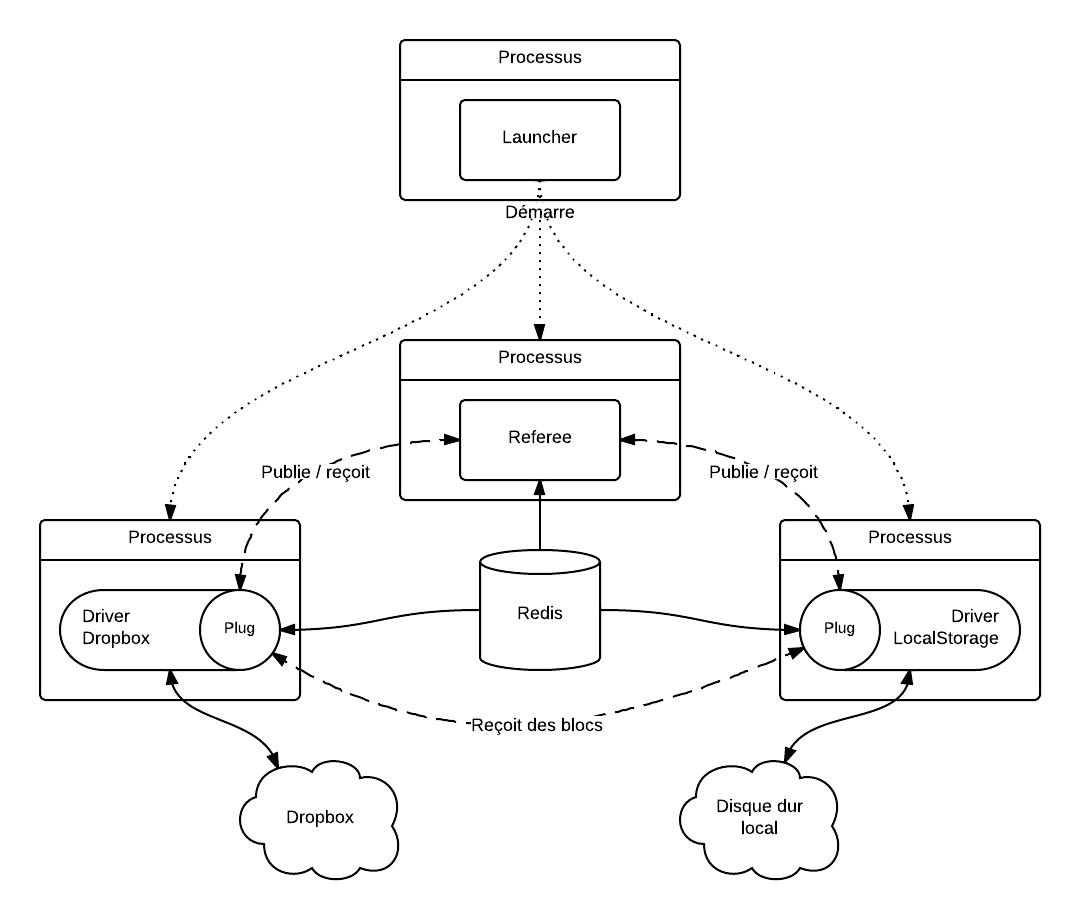
\includegraphics{global_archi.png}
\caption{Un schéma illustrant l'architecture globale d'*Onitu*, avec deux pilotes.}\label{intro:schematic}\end{figure}


\subsection{Dépendances}
\label{intro:dependencies}
Le cœur d'Onitu utilise différentes bibliothèques (d'autres dépendances existent mais sont spécifiques à certains pilotes):
\begin{description}
\item[{\href{http://circus.readthedocs.org}{Circus}}] \leavevmode
Utilisé pour pour le lancement, la gestion et la supervision des différents processus

\item[{\href{http://github.com/zeromq/pyzmq}{PyZMQ}}] \leavevmode
Une implémentation Python de la bibliothèque ZeroMQ

\item[{\href{http://github.com/andymccurdy/redis-py}{redis-py}}] \leavevmode
Une bibliothèque pour communiquer avec Redis depuis Python

\item[{\href{http://pythonhosted.org/Logbook/}{Logbook}}] \leavevmode
Une bibliothèque de journalisation, permettant à Onitu l'écriture sur un canal ZeroMQ, et rassemblant l'ensemble des journaux au même endroit.

\end{description}


\subsection{Choix techniques}
\label{intro:logbook}\label{intro:technical-choices}
Nous avons effectué quelques choix laborieux afin de construire *Onitu* dans une voie la plus efficiente et maintenable possible. Ces choix peuvent être discutables, mais en voici nos motivations:


\subsubsection{Python}
\label{intro:python}
Python est un langage polyvalent et flexible. Il fut notre premier choix, comme nous l'utilisions déjà tous et l'apprécions. Il nous permet de distribuer Onitu très facilement, sans avoir à compiler les sources ou fournir des binaires. Python est disponible sur un grand nombre de systèmes, possède de nombreuses fonctionnalités intégrées, et est simple à lire et à comprendre.

Vous aez probablement des préoccupations au niveau de la vitesse, mais *Onitu* est une application limitée par les entrées/sorties, une grande partie du temps d'exécution n'est pas dédiée à l'interprétation du code Python mais au téléchargement de fichiers ou à l'échange d'informations sur des *sockets*. Le même programme écrit dans un langage bas-niveau tel que le C serait beaucoup plus complexe, et montrerait probablement un faible gain de performances.


\subsubsection{ZeroMQ}
\label{intro:zeromq}
Onitu étant une application se basant sur de nombreux processus et exétrons, un moyen de communicatin entre ces divers fils était nécessaire. ZeroMQ est une couche du haut du protocole IP et des \emph{sockets} Unix, et fournit des patrons de messages. Onitu en utilise plusieurs, tels ROUTER/DEALER, PUBLISH/SUBSCRIBE et REQUEST/REPLY.

ZeroMQ est très rapide, disponible sur un grand nombre de plates-formes, et possède une implémentation Python. Il est plus léger et flexible que les autres acteurs du domaine, comme RabbitMQ ou ActiveMQ.


\subsubsection{Redis}
\label{intro:redis}
Onitu nécessite l'enregistrement d'informations dans une base de données persistante. Cette base doit être multiplate-forme, sans schémas, et simple à installer et maintenir. C'est dans cette optique que nous nous sommes portés sur Redis. Cependant, Redis n'est pas disponible dans la même version sur toutes les plates-formes, et n'est pas réellement persistant. Aussi, la base de données entière est chargée en mémoire, limitant donc sa taille. Ainsi, une nouvelle solution viendra sous peu remplacer *Redis*, ne répondant pas parfaitement aux besoins.


\section{Création d'un nouveau pilote}
\label{drivers:creating-a-new-driver}\label{drivers::doc}
Un pilote est un programme Python permettant la synchronisation des fichiers avec un service distant, tel Dropbox, Google Drive, SSH, FTP ou un disque local.


\subsection{Bases}
\label{drivers:basics}
Les différents pilotes communiquent avec Onitu \emph{via} la classe {\hyperref[drivers:onitu.api.Plug]{\code{Plug}}}, qui traite les opérations communes à tous les pilotes. Chaque pilote implémente ses propres tâches à l'aide du système de {\hyperref[drivers:handlers]{gestionnaires}}. Ces gestionnaires seront appelés par le {\hyperref[drivers:onitu.api.Plug]{\code{Plug}}} à diverses occasions.

Les transferts de fichiers au sein d'Onitu se font par blocs. Quand un nouveau transfert débute, le {\hyperref[drivers:onitu.api.Plug]{\code{Plug}}} demande des blocs de données aux autres pilotes, et appelle ensuite le gestionnaire \emph{upload\_chunk}.

Chaque pilote doit contenir une fonction \emph{start}, prenant un nom en premier paramètre et ne retournant rien. Le nom est choisi par l'utilisateur lors de la configuration du pilote. Cette fonction est appelée par *Onitu* au moment de l'initialisation du pilote, et ne doit pas retourner avant la fin de vie du pilote (\emph{cf} {\hyperref[drivers:onitu.api.Plug.listen]{\code{Plug.listen()}}}).

Quand un pilote détecte la mise à jour d'un fichier, il doit actualiser les {\hyperref[drivers:onitu.api.metadata.Metadata]{\code{Metadata}}} du fichier, en spécifiant une {\hyperref[drivers:onitu.api.metadata.Metadata.revision]{\code{Metadata.revision}}}, et appeler :meth.{}`.Plug.update\_file{}`.

\begin{notice}{note}{Note:}
Au cours de leur mise en service, les pilotes doivent inspecter leur système de fichiers à la recherche de créations ou mises à jour de fichiers. Ils doivent aussi écouter ces changements tout au long de leur exécution. Le méchanisme utilisé pour cela est propre à chaque pilote, et ne peut donc pas être abstrait par le {\hyperref[drivers:onitu.api.Plug]{\code{Plug}}}.
\end{notice}

Onitu fournit un ensemble de {\hyperref[contribute:tests]{\emph{tests fonctionnels}}} que vous pouvez utiliser afin de vérifier que votre pilote corresponde aux exigences.


\subsection{Gestionnaires}
\label{drivers:id1}\label{drivers:handlers}
Un gestionnaire est une fonction qui sera appelée par le \emph{Plug} à diverses occasions, comme la récupération d'un bloc de données depuis un fichier ou le lancement d'un transfert. Les pilotes peuvent définir uniquement les gestionnaires dont ils ont besoin. Par exemple, un pilote n'ayant rien de spécifique à faire à l'initialisation d'un transfert n'est pas forcé d'implémenter le gestionnaire \emph{end\_upload}. Afin d'enregistrer un gestionnaire, le décorateur {\hyperref[drivers:onitu.api.Plug.handler]{\code{Plug.handler()}}} est utilisé.

\begin{notice}{warning}{Attention:}
Tous les gestionnaires \textbf{doivent être protégés contre les accès concurrentiels}. Le \emph{Plug} utilise plusieurs exétrons pour traîter les requêtes concurrentes, et chaque gestionnaire peut ainsi être appelé depuis l'un ou l'autre de ces exétrons. Le {\hyperref[drivers:onitu.api.Plug]{\code{Plug}}} en lui-même est protégé contre les accès concurrentiels.
\end{notice}

La liste des gestionnaires pouvant être définis dans l'état actuel du projet est la suivante:
\index{get\_chunk() (built-in function)}

\begin{fulllineitems}
\phantomsection\label{drivers:get_chunk}\pysiglinewithargsret{\bfcode{get\_chunk}}{\emph{filename}, \emph{offset}, \emph{size}}{}
Retourne un bloc de données depuis un fichier, de la taille indiquée et à partir de la position données.
\begin{quote}\begin{description}
\item[{Paramètres}] \leavevmode\begin{itemize}
\item {} 
\textbf{filename} (\emph{chaîne de caractères}) -- Chemin absolu du fichier

\item {} 
\textbf{offset} (\emph{entier}) -- Position à partir de laquelle récupérer le contenu

\item {} 
\textbf{size} (\emph{entier}) -- Taille maximale du bloc de données devant être retourné

\end{itemize}

\item[{Type de retour}] \leavevmode\begin{itemize}
\item {} 
chaîne d'octets

\end{itemize}

\end{description}\end{quote}

\end{fulllineitems}

\index{upload\_chunk() (built-in function)}

\begin{fulllineitems}
\phantomsection\label{drivers:upload_chunk}\pysiglinewithargsret{\bfcode{upload\_chunk}}{\emph{filename}, \emph{offset}, \emph{chunk}}{}
Écrit un bloc de données dans un fichier, à la position indiquée.
\begin{quote}\begin{description}
\item[{Paramètres}] \leavevmode\begin{itemize}
\item {} 
\textbf{filename} (\emph{chaîne de caractères}) -- Chemin absolu du fichier

\item {} 
\textbf{offset} (\emph{entier}) -- Position à laquelle écrire le contenu

\item {} 
\textbf{chunk} (\emph{chaîne de caractères}) -- Contenu devant être écrit dans le fichier

\end{itemize}

\end{description}\end{quote}

\end{fulllineitems}

\index{start\_upload() (built-in function)}

\begin{fulllineitems}
\phantomsection\label{drivers:start_upload}\pysiglinewithargsret{\bfcode{start\_upload}}{\emph{metadata}}{}
Initialise un nouveau transfert. Le gestionnaire est appelé au lancement d'un nouveau transfert.
\begin{quote}\begin{description}
\item[{Paramètres}] \leavevmode\begin{itemize}
\item {} 
\textbf{metadata} ({\hyperref[drivers:onitu.api.metadata.Metadata]{\code{Metadata}}}) -- Métadonnées du fichier transféré

\end{itemize}

\end{description}\end{quote}

\end{fulllineitems}

\index{restart\_upload() (built-in function)}

\begin{fulllineitems}
\phantomsection\label{drivers:restart_upload}\pysiglinewithargsret{\bfcode{restart\_upload}}{\emph{metadata}, \emph{offset}}{}
Relance un transfert défectueux. Ce gestionnaire sera appelé au lancement si un transfert a été stoppé.
\begin{quote}\begin{description}
\item[{Paramètres}] \leavevmode\begin{itemize}
\item {} 
\textbf{metadata} ({\hyperref[drivers:onitu.api.metadata.Metadata]{\code{Metadata}}}) -- Métadonnées du fichier transféré

\item {} 
\textbf{offset} (\emph{entier}) -- La position du dernier bloc envoyé

\end{itemize}

\end{description}\end{quote}

\end{fulllineitems}

\index{end\_upload() (built-in function)}

\begin{fulllineitems}
\phantomsection\label{drivers:end_upload}\pysiglinewithargsret{\bfcode{end\_upload}}{\emph{metadata}}{}
Appelé lorsqu'un transfert est terminé.
\begin{quote}\begin{description}
\item[{Paramètres}] \leavevmode\begin{itemize}
\item {} 
\textbf{metadata} ({\hyperref[drivers:onitu.api.metadata.Metadata]{\code{Metadata}}}) -- Métadonnées du fichier transféré

\end{itemize}

\end{description}\end{quote}

\end{fulllineitems}

\index{abort\_upload() (built-in function)}

\begin{fulllineitems}
\phantomsection\label{drivers:abort_upload}\pysiglinewithargsret{\bfcode{abort\_upload}}{\emph{metadata}}{}
Appelé lorsqu'un transfert est annulé. Cela peut arriver par exemple si une nouvelle version du fichier apparaît pendant le transfert.
\begin{quote}\begin{description}
\item[{Paramètres}] \leavevmode\begin{itemize}
\item {} 
\textbf{metadata} ({\hyperref[drivers:onitu.api.metadata.Metadata]{\code{Metadata}}}) -- Métadonnées du fichier transféré

\end{itemize}

\end{description}\end{quote}

\end{fulllineitems}



\subsection{Plug}
\label{drivers:the-plug}\index{Plug (class in onitu.api)}

\begin{fulllineitems}
\phantomsection\label{drivers:onitu.api.Plug}\pysigline{\strong{class }\code{onitu.api.}\bfcode{Plug}}
Le \emph{Plug} est la méthode privilégiée pour un pilote de communiquer avec un autre pilote, le {\hyperref[components:onitu.referee.Referee]{\code{Referee}}} ou la base de données.

Chaque pilote doit instancier un nouveau \emph{Plug} et en définir les gestionnaires (voir {\hyperref[drivers:onitu.api.Plug.handler]{\code{handler()}}}).

{\hyperref[drivers:onitu.api.Plug.initialize]{\code{initialize()}}} doit être appelée au début de la fonction \emph{start}. Une fois que le pilote est prêt à recevoir des requêtes depuis les autres pilotes, il doit appeler {\hyperref[components:onitu.referee.Referee.listen]{\code{listen()}}}. Cette fonction bloque jusqu'à ce que le pilote soit fermé.
\index{get\_metadata() (onitu.api.Plug method)}

\begin{fulllineitems}
\phantomsection\label{drivers:onitu.api.Plug.get_metadata}\pysiglinewithargsret{\bfcode{get\_metadata}}{\emph{filename}}{}~\begin{quote}\begin{description}
\item[{Paramètres}] \leavevmode\begin{itemize}
\item {} 
\textbf{filename} -- Le nom du fichier, avec son chemin absolu depuis la racine du pilote

\end{itemize}

\item[{Type de retour}] \leavevmode\begin{itemize}
\item {} 
{\hyperref[drivers:onitu.api.metadata.Metadata]{\code{Metadata}}}

\end{itemize}

\end{description}\end{quote}

Si le fichier n'existe pas dans *Onitu*, il sera créé lors de l'appel à {\hyperref[drivers:onitu.api.metadata.Metadata.write]{\code{Metadata.write()}}}.

\end{fulllineitems}

\index{handler() (onitu.api.Plug method)}

\begin{fulllineitems}
\phantomsection\label{drivers:onitu.api.Plug.handler}\pysiglinewithargsret{\bfcode{handler}}{\emph{task=None}}{}
Décorateur utilisé pour enregistrer un gestionnaire pour une tâche particulière.
\begin{quote}\begin{description}
\item[{Paramètres}] \leavevmode\begin{itemize}
\item {} 
\textbf{task} (\emph{chaîne de caractères}) -- Optionnel. Nom du gestionnaire. Si non spécifié, le nom de la fonction sera utilisé.

\end{itemize}

\end{description}\end{quote}

Exemple:

\begin{Verbatim}[commandchars=\\\{\}]
\PYG{n+nd}{@plug.handler}\PYG{p}{(}\PYG{p}{)}
\PYG{k}{def} \PYG{n+nf}{get\PYGZus{}chunk}\PYG{p}{(}\PYG{n}{filename}\PYG{p}{,} \PYG{n}{offset}\PYG{p}{,} \PYG{n}{size}\PYG{p}{)}\PYG{p}{:}
    \PYG{k}{with} \PYG{n+nb}{open}\PYG{p}{(}\PYG{n}{filename}\PYG{p}{,} \PYG{l+s}{\PYGZsq{}}\PYG{l+s}{rb}\PYG{l+s}{\PYGZsq{}}\PYG{p}{)} \PYG{k}{as} \PYG{n}{f}\PYG{p}{:}
        \PYG{n}{f}\PYG{o}{.}\PYG{n}{seek}\PYG{p}{(}\PYG{n}{offset}\PYG{p}{)}
        \PYG{k}{return} \PYG{n}{f}\PYG{o}{.}\PYG{n}{read}\PYG{p}{(}\PYG{n}{size}\PYG{p}{)}
\end{Verbatim}

\end{fulllineitems}

\index{initialize() (onitu.api.Plug method)}

\begin{fulllineitems}
\phantomsection\label{drivers:onitu.api.Plug.initialize}\pysiglinewithargsret{\bfcode{initialize}}{\emph{name}}{}
Initialise les différents composants du \emph{Plug}. Le pilote doit l'appeler au début de la fonction \emph{start}.
\begin{quote}\begin{description}
\item[{Paramètres}] \leavevmode\begin{itemize}
\item {} 
\textbf{name} (\emph{chaîne de caractères}) -- Nom de l'entrée courante, comme donné à la fonction \emph{start}.

\end{itemize}

\end{description}\end{quote}

\end{fulllineitems}

\index{listen() (onitu.api.Plug method)}

\begin{fulllineitems}
\phantomsection\label{drivers:onitu.api.Plug.listen}\pysiglinewithargsret{\bfcode{listen}}{\emph{wait=True}}{}
Lance l'écoute des requêtes en provenance des autres pilotes ou du
{\hyperref[components:onitu.referee.Referee]{\code{Referee}}}.
\begin{quote}\begin{description}
\item[{Paramètres}] \leavevmode\begin{itemize}
\item {} 
\textbf{wait} (\emph{booléen}) -- Optionnel. Si \emph{True}, bloque jusqu'à ce que le \emph{Plug} se termine. Par défaut à \emph{True}.

\end{itemize}

\end{description}\end{quote}

Cette méthode lance deux exétrons:
\begin{itemize}
\item {} \index{Plug.Router (class in onitu.api.router)}

\begin{fulllineitems}
\phantomsection\label{drivers:onitu.api.router.Plug.Router}\pysiglinewithargsret{\strong{class }\bfcode{Router}}{\emph{plug}}{}
Reçoit et répond aux requêtes provenant des autres pilotes. C'est ce composant qui appelle le gestionnaire \emph{get\_chunk}. Il utilise un seul fil d'exécution, ce qui signifie qu'une seul appel à \emph{get\_chunk} peut être réalisé simultanément.

\end{fulllineitems}


\item {} \index{Dealer (class in onitu.api.dealer)}

\begin{fulllineitems}
\phantomsection\label{drivers:onitu.api.dealer.Dealer}\pysiglinewithargsret{\strong{class }\code{onitu.api.dealer.}\bfcode{Dealer}}{\emph{plug}}{}
Reçoit et répond aux ordres provenant du \emph{Referee}.

Toutes les requêtes sont traitées dans une file d'exétrons.

\end{fulllineitems}


\end{itemize}

\end{fulllineitems}

\index{update\_file() (onitu.api.Plug method)}

\begin{fulllineitems}
\phantomsection\label{drivers:onitu.api.Plug.update_file}\pysiglinewithargsret{\code{Plug.}\bfcode{update\_file}}{\emph{metadata}}{}
Cette méthode doit être appelée par le pilote après chaque création ou mise à jour de fichier. Elle prend en paramètre un objet {\hyperref[drivers:onitu.api.metadata.Metadata]{\code{Metadata}}} contenant les nouvelles valeurs des propriétés du fichier.

\end{fulllineitems}


\end{fulllineitems}



\subsection{Metadata}
\label{drivers:metadata}\index{Metadata (class in onitu.api.metadata)}

\begin{fulllineitems}
\phantomsection\label{drivers:onitu.api.metadata.Metadata}\pysiglinewithargsret{\strong{class }\code{onitu.api.metadata.}\bfcode{Metadata}}{\emph{plug=None}, \emph{filename=None}, \emph{size=0}}{}
The Metadata class represent the metadata of any file in Onitu.

This class should always be instantiated via the
{\hyperref[drivers:onitu.api.metadata.Metadata.get_by_id]{\code{get\_by\_id()}}} or {\hyperref[drivers:onitu.api.metadata.Metadata.get_by_filename]{\code{get\_by\_filename()}}}
class methods.
However, the drivers should never instantiate a new
{\hyperref[drivers:onitu.api.metadata.Metadata]{\code{Metadata}}} object themselves, but use the
{\hyperref[drivers:onitu.api.Plug.get_metadata]{\code{Plug.get\_metadata()}}} function.

The attributes available for each file are the following :
\begin{description}
\item[{\textbf{filename}}] \leavevmode
The absolute filename of the file

\item[{\textbf{size}}] \leavevmode
The size of the file, in octets

\item[{\textbf{revision}}] \leavevmode
This field is specific to each entry. It is a string
representing the current revision of the file for the
current entry.
The drivers should compare an upstream and a local version
of a file with this field. The format is dependant from the
driver (it can be whatever you want: a timestamp, a number,
a hash...).

\item[{\textbf{owners}}] \leavevmode
The entries which should have this file

\item[{\textbf{uptodate}}] \leavevmode
The entries with an up-to-date version of this file

\end{description}
\index{get\_by\_filename() (onitu.api.metadata.Metadata class method)}

\begin{fulllineitems}
\phantomsection\label{drivers:onitu.api.metadata.Metadata.get_by_filename}\pysiglinewithargsret{\strong{classmethod }\bfcode{get\_by\_filename}}{\emph{plug}, \emph{filename}}{}
Instantiate a new {\hyperref[drivers:onitu.api.metadata.Metadata]{\code{Metadata}}} object for the file
with the given name.

\end{fulllineitems}

\index{get\_by\_id() (onitu.api.metadata.Metadata class method)}

\begin{fulllineitems}
\phantomsection\label{drivers:onitu.api.metadata.Metadata.get_by_id}\pysiglinewithargsret{\strong{classmethod }\bfcode{get\_by\_id}}{\emph{plug}, \emph{fid}}{}
Instantiate a new {\hyperref[drivers:onitu.api.metadata.Metadata]{\code{Metadata}}} object for the file
with the given id.

\end{fulllineitems}

\index{revision (onitu.api.metadata.Metadata attribute)}

\begin{fulllineitems}
\phantomsection\label{drivers:onitu.api.metadata.Metadata.revision}\pysigline{\bfcode{revision}}
The revision of a file can be any string, and should be
used to compare the different versions of a file on driver.

Each driver can use its own system of revisions, as it is
stored for each entry.

\end{fulllineitems}

\index{write() (onitu.api.metadata.Metadata method)}

\begin{fulllineitems}
\phantomsection\label{drivers:onitu.api.metadata.Metadata.write}\pysiglinewithargsret{\bfcode{write}}{}{}
Write the metadata of the current file in the database.

\end{fulllineitems}

\index{write\_revision() (onitu.api.metadata.Metadata method)}

\begin{fulllineitems}
\phantomsection\label{drivers:onitu.api.metadata.Metadata.write_revision}\pysiglinewithargsret{\bfcode{write\_revision}}{}{}
Write the current revision in the database. Called
by {\hyperref[drivers:onitu.api.metadata.Metadata.write]{\code{write()}}}.

\end{fulllineitems}


\end{fulllineitems}



\subsection{Example}
\label{drivers:example}
Usually, the drivers are created as a set of functions in a single file, with the Plug in a global variable. However, you can use a different style if you want, such as a class.

Here is an example of a simple driver working with the local file system :

\begin{Verbatim}[commandchars=\\\{\},numbers=left,firstnumber=1,stepnumber=1]
\PYG{k+kn}{import} \PYG{n+nn}{os}

\PYG{k+kn}{from} \PYG{n+nn}{onitu.api} \PYG{k+kn}{import} \PYG{n}{Plug}

\PYG{c}{\PYGZsh{} A dummy library supposed to watch the file system}
\PYG{k+kn}{from} \PYG{n+nn}{fsmonitor} \PYG{k+kn}{import} \PYG{n}{FSWatcher}

\PYG{n}{plug} \PYG{o}{=} \PYG{n}{Plug}\PYG{p}{(}\PYG{p}{)}


\PYG{n+nd}{@plug.handler}\PYG{p}{(}\PYG{p}{)}
\PYG{k}{def} \PYG{n+nf}{get\PYGZus{}chunk}\PYG{p}{(}\PYG{n}{filename}\PYG{p}{,} \PYG{n}{offset}\PYG{p}{,} \PYG{n}{size}\PYG{p}{)}\PYG{p}{:}
    \PYG{k}{with} \PYG{n+nb}{open}\PYG{p}{(}\PYG{n}{filename}\PYG{p}{,} \PYG{l+s}{\PYGZsq{}}\PYG{l+s}{rb}\PYG{l+s}{\PYGZsq{}}\PYG{p}{)} \PYG{k}{as} \PYG{n}{f}\PYG{p}{:}
        \PYG{n}{f}\PYG{o}{.}\PYG{n}{seek}\PYG{p}{(}\PYG{n}{offset}\PYG{p}{)}
        \PYG{k}{return} \PYG{n}{f}\PYG{o}{.}\PYG{n}{read}\PYG{p}{(}\PYG{n}{size}\PYG{p}{)}


\PYG{n+nd}{@plug.handler}\PYG{p}{(}\PYG{p}{)}
\PYG{k}{def} \PYG{n+nf}{upload\PYGZus{}chunk}\PYG{p}{(}\PYG{n}{filename}\PYG{p}{,} \PYG{n}{offset}\PYG{p}{,} \PYG{n}{chunk}\PYG{p}{)}\PYG{p}{:}
    \PYG{k}{with} \PYG{n+nb}{open}\PYG{p}{(}\PYG{n}{filename}\PYG{p}{,} \PYG{l+s}{\PYGZsq{}}\PYG{l+s}{ab}\PYG{l+s}{\PYGZsq{}}\PYG{p}{)} \PYG{k}{as} \PYG{n}{f}\PYG{p}{:}
        \PYG{n}{f}\PYG{o}{.}\PYG{n}{seek}\PYG{p}{(}\PYG{n}{offset}\PYG{p}{)}
        \PYG{n}{f}\PYG{o}{.}\PYG{n}{write}\PYG{p}{(}\PYG{n}{chunk}\PYG{p}{)}


\PYG{n+nd}{@plug.handler}\PYG{p}{(}\PYG{p}{)}
\PYG{k}{def} \PYG{n+nf}{end\PYGZus{}upload}\PYG{p}{(}\PYG{n}{metadata}\PYG{p}{)}\PYG{p}{:}
    \PYG{n}{metadata}\PYG{o}{.}\PYG{n}{revision} \PYG{o}{=} \PYG{n}{os}\PYG{o}{.}\PYG{n}{path}\PYG{o}{.}\PYG{n}{getmtime}\PYG{p}{(}\PYG{n}{metadata}\PYG{o}{.}\PYG{n}{filename}\PYG{p}{)}
    \PYG{n}{metadata}\PYG{o}{.}\PYG{n}{write\PYGZus{}revision}\PYG{p}{(}\PYG{p}{)}


\PYG{k}{class} \PYG{n+nc}{Watcher}\PYG{p}{(}\PYG{n}{FSWatcher}\PYG{p}{)}\PYG{p}{:}
    \PYG{k}{def} \PYG{n+nf}{on\PYGZus{}update}\PYG{p}{(}\PYG{n+nb+bp}{self}\PYG{p}{,} \PYG{n}{filename}\PYG{p}{)}\PYG{p}{:}
        \PYG{l+s+sd}{\PYGZdq{}\PYGZdq{}\PYGZdq{}Called each time an update of a file is detected}
\PYG{l+s+sd}{        \PYGZdq{}\PYGZdq{}\PYGZdq{}}
        \PYG{n}{metadata} \PYG{o}{=} \PYG{n}{plug}\PYG{o}{.}\PYG{n}{get\PYGZus{}metadata}\PYG{p}{(}\PYG{n}{filename}\PYG{p}{)}
        \PYG{n}{metadata}\PYG{o}{.}\PYG{n}{revision} \PYG{o}{=} \PYG{n}{os}\PYG{o}{.}\PYG{n}{path}\PYG{o}{.}\PYG{n}{getmtime}\PYG{p}{(}\PYG{n}{metadata}\PYG{o}{.}\PYG{n}{filename}\PYG{p}{)}
        \PYG{n}{metadata}\PYG{o}{.}\PYG{n}{size} \PYG{o}{=} \PYG{n}{os}\PYG{o}{.}\PYG{n}{path}\PYG{o}{.}\PYG{n}{getsize}\PYG{p}{(}\PYG{n}{metadata}\PYG{o}{.}\PYG{n}{filename}\PYG{p}{)}
        \PYG{n}{plug}\PYG{o}{.}\PYG{n}{update\PYGZus{}file}\PYG{p}{(}\PYG{n}{metadata}\PYG{p}{)}

    \PYG{k}{def} \PYG{n+nf}{check\PYGZus{}changes}\PYG{p}{(}\PYG{n+nb+bp}{self}\PYG{p}{)}\PYG{p}{:}
        \PYG{l+s+sd}{\PYGZdq{}\PYGZdq{}\PYGZdq{}Check the changes on the file system since the last launch}
\PYG{l+s+sd}{        \PYGZdq{}\PYGZdq{}\PYGZdq{}}
        \PYG{k}{for} \PYG{n}{filename} \PYG{o+ow}{in} \PYG{n+nb+bp}{self}\PYG{o}{.}\PYG{n}{files}\PYG{p}{:}
            \PYG{n}{revision} \PYG{o}{=} \PYG{n}{os}\PYG{o}{.}\PYG{n}{path}\PYG{o}{.}\PYG{n}{getmtime}\PYG{p}{(}\PYG{n}{filename}\PYG{p}{)}
            \PYG{n}{metadata} \PYG{o}{=} \PYG{n}{plug}\PYG{o}{.}\PYG{n}{get\PYGZus{}metadata}\PYG{p}{(}\PYG{n}{filename}\PYG{p}{)}

            \PYG{c}{\PYGZsh{} If the file is more recent}
            \PYG{k}{if} \PYG{n}{revision} \PYG{o}{\PYGZgt{}} \PYG{n}{metadata}\PYG{o}{.}\PYG{n}{revision}\PYG{p}{:}
                \PYG{n}{metadata}\PYG{o}{.}\PYG{n}{revision} \PYG{o}{=} \PYG{n}{os}\PYG{o}{.}\PYG{n}{path}\PYG{o}{.}\PYG{n}{getmtime}\PYG{p}{(}\PYG{n}{metadata}\PYG{o}{.}\PYG{n}{filename}\PYG{p}{)}
                \PYG{n}{metadata}\PYG{o}{.}\PYG{n}{size} \PYG{o}{=} \PYG{n}{os}\PYG{o}{.}\PYG{n}{path}\PYG{o}{.}\PYG{n}{getsize}\PYG{p}{(}\PYG{n}{metadata}\PYG{o}{.}\PYG{n}{filename}\PYG{p}{)}
                \PYG{n}{plug}\PYG{o}{.}\PYG{n}{update\PYGZus{}file}\PYG{p}{(}\PYG{n}{metadata}\PYG{p}{)}


\PYG{k}{def} \PYG{n+nf}{start}\PYG{p}{(}\PYG{o}{*}\PYG{n}{args}\PYG{p}{,} \PYG{o}{*}\PYG{o}{*}\PYG{n}{kwargs}\PYG{p}{)}\PYG{p}{:}
    \PYG{n}{plug}\PYG{o}{.}\PYG{n}{initialize}\PYG{p}{(}\PYG{o}{*}\PYG{n}{args}\PYG{p}{,} \PYG{o}{*}\PYG{o}{*}\PYG{n}{kwargs}\PYG{p}{)}

    \PYG{n}{root} \PYG{o}{=} \PYG{n}{plug}\PYG{o}{.}\PYG{n}{options}\PYG{p}{[}\PYG{l+s}{\PYGZsq{}}\PYG{l+s}{root}\PYG{l+s}{\PYGZsq{}}\PYG{p}{]}
    \PYG{n}{os}\PYG{o}{.}\PYG{n}{chdir}\PYG{p}{(}\PYG{n}{root}\PYG{p}{)}

    \PYG{n}{watcher} \PYG{o}{=} \PYG{n}{Watcher}\PYG{p}{(}\PYG{n}{root}\PYG{p}{)}
    \PYG{n}{watcher}\PYG{o}{.}\PYG{n}{check\PYGZus{}changes}\PYG{p}{(}\PYG{p}{)}
    \PYG{n}{watcher}\PYG{o}{.}\PYG{n}{start}\PYG{p}{(}\PYG{p}{)}

    \PYG{n}{plug}\PYG{o}{.}\PYG{n}{listen}\PYG{p}{(}\PYG{p}{)}
\end{Verbatim}


\section{Components documentation}
\label{components::doc}\label{components:components-documentation}
Here is the documentation of the parts not covered yet. You should not have to worry about those parts if you are writing a new driver, but they can be very useful if you want to hack the core of Onitu.


\subsection{Launcher}
\label{components:launcher}\label{components:module-onitu.__main__}\index{onitu.\_\_main\_\_ (module)}
This module starts Onitu. It does the following:
\begin{itemize}
\item {} 
parse the command line options

\item {} 
configure the logger

\item {} 
parse the setup

\item {} 
clean the database

\item {} 
launch the different elements using the Circus library

\end{itemize}
\index{get\_logs\_dispatcher() (in module onitu.\_\_main\_\_)}

\begin{fulllineitems}
\phantomsection\label{components:onitu.__main__.get_logs_dispatcher}\pysiglinewithargsret{\code{onitu.\_\_main\_\_.}\bfcode{get\_logs\_dispatcher}}{\emph{uri=None}, \emph{debug=False}}{}
Configure the dispatcher that will print the logs received
on the ZeroMQ channel.

\end{fulllineitems}

\index{start\_setup() (in module onitu.\_\_main\_\_)}

\begin{fulllineitems}
\phantomsection\label{components:onitu.__main__.start_setup}\pysiglinewithargsret{\code{onitu.\_\_main\_\_.}\bfcode{start\_setup}}{\emph{*args}, \emph{**kwargs}}{}
Parse the setup JSON file, clean the database,
and start the {\hyperref[components:onitu.referee.Referee]{\code{Referee}}} and the drivers.

\end{fulllineitems}

\index{start\_watcher() (in module onitu.\_\_main\_\_)}

\begin{fulllineitems}
\phantomsection\label{components:onitu.__main__.start_watcher}\pysiglinewithargsret{\code{onitu.\_\_main\_\_.}\bfcode{start\_watcher}}{\emph{*args}, \emph{**kwargs}}{}
Start a Circus Watcher.
If a command is already running, we try again.

\end{fulllineitems}



\subsection{Referee}
\label{components:referee}
The role of the Referee is to receive the events emitted by the drivers, and to send notifications to the other drivers accordingly to the configuration rules.
\index{Referee (class in onitu.referee)}

\begin{fulllineitems}
\phantomsection\label{components:onitu.referee.Referee}\pysigline{\strong{class }\code{onitu.referee.}\bfcode{Referee}}
Referee class, receive all events and deal with them.

The events are represented as Redis List `events' that should be
appended with RPUSH. Each item is the file id (fid) of the file
which triggered the event.

The Referee give orders to the entries via his PUB ZMQ socket,
whose port is stored in the Redis `referee:publisher' key.
The Plug of each entry should subscribe to this port with a PULL
socket and subscribe to all the events starting by their name.

The notifications are sent to the publishers as multipart
messages with three parts :
\begin{itemize}
\item {} 
The name of the addressee (the channel)

\item {} 
The name of the entry from which the file should be transferred

\item {} 
The id of the file

\end{itemize}
\index{listen() (onitu.referee.Referee method)}

\begin{fulllineitems}
\phantomsection\label{components:onitu.referee.Referee.listen}\pysiglinewithargsret{\bfcode{listen}}{}{}
Listen to all the events, and handle them

\end{fulllineitems}


\end{fulllineitems}



\subsection{Utils}
\label{components:utils}\label{components:module-onitu.utils}\index{onitu.utils (module)}
This module provides a set of classes and functions useful in several
parts of Onitu.
\index{Redis (class in onitu.utils)}

\begin{fulllineitems}
\phantomsection\label{components:onitu.utils.Redis}\pysiglinewithargsret{\strong{class }\code{onitu.utils.}\bfcode{Redis}}{\emph{*args}, \emph{**kwargs}}{}
This is a simple wrapper around the \code{redis.Redis} object
from the redis-py library.

It adds a \code{session} attribute, which can be used as a
standard \code{redis.Redis} object, but will prefix every key
by the current session-key.

This session key is used by Onitu to separate the different
sessions in the database. As Redis only handles a small finite
number of databases, we use a single database, but prefix all the
keys.

The session attribute should always be used.

\end{fulllineitems}

\index{connect\_to\_redis() (in module onitu.utils)}

\begin{fulllineitems}
\phantomsection\label{components:onitu.utils.connect_to_redis}\pysiglinewithargsret{\code{onitu.utils.}\bfcode{connect\_to\_redis}}{\emph{*args}, \emph{**kwargs}}{}
This class return a new {\hyperref[components:onitu.utils.Redis]{\code{Redis}}} object, ready to
receive requests, with the session enabled.
It blocks until the connection is made.

You can pass extra arguments to the {\hyperref[components:onitu.utils.Redis]{\code{Redis}}} class by
giving them to this function.

\end{fulllineitems}



\section{Contributing to Onitu}
\label{contribute:contributing-to-onitu}\label{contribute::doc}
Onitu is an opensource project, all of our codebase is available on Github and we would be very happy to include fixes or features from the comunity.

Here are some guidelines on what to look out for if you are hacking the code or having issues.


\subsection{Reporting issues}
\label{contribute:reporting-issues}
When you encounter an issue with Onitu we'dd love to hear about it. Not that we particularly like having problems with the codebase, but its better to fix them than to leave them in there.
If you submit a bug report please include all the information available to you, here are some things you can do:
\begin{itemize}
\item {} 
If the problem is reproductible you can restart Onitu in debugging mode.

\item {} 
Onitu generate logging output, this is very usefull to us.

\item {} 
Try to simplify the things you are doing until getting a minimal set of actions reproducing the problem.

\end{itemize}


\subsection{Running the tests}
\label{contribute:tests}\label{contribute:running-the-tests}
If you developed a new feature or simply want to try out an instalation of Onitu you can run the unit tests. For this you will need to install the requirements for the testing framework, this can easily be done using:
\begin{itemize}
\item {} 
\emph{pip install -r requirements\_dev.txt}

\end{itemize}

The unit tests can be launched by the command \emph{py.test tests/}. You can also use \emph{tox} in order to automatically generate a clean and functionnal environment for executing the tests.

Finnaly, some environment variables are useful to execute the tests, they are:
\begin{quote}
\begin{description}
\item[{ONITU\_TEST\_TIME\_UNIT}] \leavevmode
Many tests are based on timeout to consider a transfer as failed. This variable contains thus a number of seconds corresponding to a time unit, \emph{1s} by default.

\item[{ONITU\_TEST\_DRIVER}] \leavevmode
The tests set is only executed for one driver at a time. This variable is used to determine which driver will be tested, and can contains values such as \emph{local\_storage} or \emph{ssh}.

\end{description}
\end{quote}


\subsection{Good practices with Git}
\label{contribute:good-practices-with-git}
In order to maintain the project while including contributions from the opensource comunity we need to have some rules in place. This is especialy true with regard to the use of Git.

When developing new features this should always be done on feature branches that are dedicated to that particular feature. Once the feature is ready, the feature branch should be rebased on the current develop branch before doing a pull request.

The maintainers of the develop branch will then review the pull request and merge it into develop when its ready. They might ask you to do some changes beforehand.

You should never merge master onto your feature branch, instead always use rebase on local code.


\subsection{Coding style}
\label{contribute:coding-style}
The code you contribute to the project should respect the guidelines defined in \index{Python Enhancement Proposals!PEP 008}\href{http://www.python.org/dev/peps/pep-0008}{\textbf{PEP 008}}, you can use a tool such as flake8 to check if this is the case. In case you're wondering: we use four spaces indentation.

Please take those rules into account, we aim to have a clean codebase and codestyle is a big part of that. Your code will be checked when we consider your pull requests.


\section{Changelog}
\label{changelog::doc}\label{changelog:changelog}
You can find a detailed summary of the changes between the releases on \href{https://github.com/onitu/onitu/releases}{Github}. Here is a brief summary :


\subsection{0.1}
\label{changelog:id1}
First release.

The Referee can handle simple rules based on the path, the size and the file extension.

Four drivers are available :
\begin{itemize}
\item {} 
Local storage

\item {} 
Dropbox

\item {} 
Google Drive

\item {} 
SSH

\end{itemize}

The test suite cover the Referee and the drivers. Some benchmarks are available.


\chapter{Indices and tables}
\label{index:indices-and-tables}\begin{itemize}
\item {} 
\emph{genindex}

\item {} 
\emph{modindex}

\item {} 
\emph{search}

\end{itemize}


\renewcommand{\indexname}{Python Module Index}
\begin{theindex}
\def\bigletter#1{{\Large\sffamily#1}\nopagebreak\vspace{1mm}}
\bigletter{o}
\item {\texttt{onitu.\_\_main\_\_}}, \pageref{components:module-onitu.__main__}
\item {\texttt{onitu.utils}}, \pageref{components:module-onitu.utils}
\end{theindex}

\renewcommand{\indexname}{Index}
\printindex
\end{document}
